\section{Proposed Lightweight Model}
\label{sec:proposed_model}

Rather than designing a new architecture from scratch, we adopt a systematic \emph{selection-and-adaptation} approach. A broad pool of existing lightweight and efficient architectures is fine-tuned under a largely shared training protocol, with the deviations documented below, on the AvocadoLeaf dataset, and the best-performing candidate under joint accuracy-size-latency constraints is proposed as the deployment model for this task (Section~\ref{sec:experiments}). This section describes the candidate pool, the transfer-learning strategy applied to each, and the shared training protocol.

\subsection{Candidate Architectures}

We evaluate 15 architectures spanning five groups (a finer split of the three broader CNN / hybrid CNN-Transformer / pure-transformer families referenced in Section~\ref{sec:related_work}):
\begin{enumerate}
    \item[(1)] a Vanilla CNN trained from scratch as a minimal baseline.
    \item[(2)] a ResNet-18 \citep{he2016deep} baseline.
    \item[(3)] mobile-oriented CNNs (MobileNet-V2 \citep{sandler2018mobilenetv2}, MobileNet-V4 \citep{qin2024mobilenetv4}, TinyNet \citep{han2020tinynet}, GhostNet-V2 \citep{tang2022ghostnetv2}, EfficientNet-B0 \citep{tan2019efficientnet}).
    \item[(4)] hybrid CNN-Transformer designs (MobileOne \citep{vasu2023mobileone}, EdgeNeXt \citep{maaz2022edgenext}, FastViT \citep{vasu2023fastvit}, EfficientViT \citep{liu2023efficientvit}, ConvNeXt-V1 \citep{liu2022convnet}, ConvNeXt-V2 \citep{woo2023convnextv2}).
    \item[(5)] pure vision transformers (ViT-B/16 \citep{dosovitskiy2021vit}, SwinTransformer \citep{liu2021swin}).
\end{enumerate}
All architectures except Vanilla CNN are initialised from ImageNet-pretrained weights obtained from \texttt{torchvision} or \texttt{timm}.

\subsection{Transfer-Learning Strategy}

Because the AvocadoLeaf training set is comparatively small (1,302 training images across six classes), fully fine-tuning all layers of large pretrained backbones risks overfitting. We therefore apply \emph{selective layer unfreezing}. For every pretrained model, all backbone weights are frozen except the last one to two stages (or the last two encoder layers, for the transformer-based models) and a newly initialised classification head sized to the six AvocadoLeaf classes. Table~\ref{tab:finetune_strategy} summarises the unfreezing strategy per architecture family. The Vanilla CNN baseline has no pretrained weights and is instead trained end-to-end from random initialisation.

\begin{table*}[htbp]
\centering
\caption{Transfer-learning strategy by architecture family.}
\label{tab:finetune_strategy}
\small
\begin{tabularx}{\textwidth}{l X l}
\toprule
\textbf{Architecture family} & \textbf{Members} & \textbf{Unfrozen layers} \\
\midrule
Vanilla CNN & -- & All (trained from scratch) \\
ResNet-18 & -- & \texttt{layer4} + classifier head \\
Mobile CNNs & MobileNet-V2, MobileNet-V4, TinyNet, GhostNet-V2, EfficientNet-B0 & Last 2 feature blocks + head \\
Hybrid CNN-Transformer & MobileOne, EdgeNeXt, FastViT, EfficientViT, ConvNeXt-V1, ConvNeXt-V2 & Last 2 stages + head \\
Vision Transformers & ViT-B/16, SwinTransformer & Last 2 encoder layers + head \\
\bottomrule
\end{tabularx}
\end{table*}

\subsection{Training Protocol}

All 15 models share the same optimiser, learning-rate schedule, epoch budget, and data augmentation policy, using AdamW (learning rate $1\times10^{-4}$, weight decay $1\times10^{-4}$) with cosine-annealing decay over a maximum of 100 epochs, cross-entropy loss, and early stopping with a patience of 5 epochs on validation loss. Input images are resized to $224\times224$ and normalised using ImageNet statistics. Training-time data augmentation consists of random-resized cropping (scale $0.6$–$1.0$), horizontal flipping, random rotation ($\pm15^\circ$, applied with probability 0.3), colour jittering (brightness/contrast/saturation/hue), and random erasing. Models are always evaluated without augmentation at validation and test time.

Two aspects of this protocol are not held perfectly constant across all 15 candidates. First, the unfrozen-layer depth in Table~\ref{tab:finetune_strategy} differs between ResNet-18 (one stage) and the remaining pretrained models (two stages or encoder layers). Second, despite the augmentation policy above being intended uniformly, the ConvNeXt-V2/BoVien checkpoint reported in Section~\ref{sec:experiments} was in fact trained with augmentation disabled, and this switch was not applied consistently across all candidates. The ablation study (Section~\ref{subsec:ablation}) examines its effect on BoVien directly. See the Limitations discussion (Section~\ref{sec:discussion}) for further detail on both points.

The architecture that achieves the best joint accuracy-size-latency trade-off under this protocol, ConvNeXt-V2, is adopted as our proposed lightweight model for avocado disease classification. The full comparison against the other 14 candidates is reported in Section~\ref{sec:experiments}.

\subsection{Proposed Model Architecture}
\label{subsec:proposed_architecture}

As introduced in Section~\ref{sec:introduction}, we name the resulting deployment model \textbf{BoVien}, the \texttt{convnextv2\_atto} variant of ConvNeXt-V2 (3.7M parameters with its original 1000-way ImageNet head, 0.55 GFLOPs at $224\times224$), the smallest in the ConvNeXt-V2 family, adapted to AvocadoLeaf via the selective layer unfreezing strategy of Table~\ref{tab:finetune_strategy}. Replacing this head with the six-way AvocadoLeaf classification head used throughout this paper brings the parameter count down to the 3.4M reported in Table~\ref{tab:arch_compare}. Figure~\ref{fig:proposed_architecture} details its architecture. Box width encodes channel count, and box height/depth encode spatial resolution. Each stage's internals are grouped into a single box instead of listing every submodule. Reading left to right, a $4\times4$/stride-4 convolutional stem produces a $56\times56\times40$ feature map, which then passes through four stages of ConvNeXt-V2 blocks (depths 2-2-6-2, widths 40-80-160-320) with $2\times2$ downsampling between stages, ending at $7\times7\times320$. This is visible in the figure as boxes that shrink in height/depth (spatial resolution) while growing in length (channel count). Following Table~\ref{tab:finetune_strategy}, Stages~1-2 (grey) remain frozen at their ImageNet-pretrained weights, while Stages~3-4 (orange) are fine-tuned on AvocadoLeaf. Each stage is a stack of ConvNeXt-V2 blocks, each consisting of a $7\times7$ depthwise convolution, LayerNorm, an inverted-bottleneck MLP ($C\!\to\!4C\!\to\!C$) with GELU activation, and Global Response Normalisation (GRN) inserted between the two pointwise layers (the modification that distinguishes ConvNeXt-V2 from ConvNeXt-V1's LayerScale-based block), the whole block wrapped in a residual connection. The classification head (global average pool $\to$ LayerNorm $\to$ linear) is entirely new (green) and pools the $320$-d backbone feature, mapping it to a probability over the six AvocadoLeaf classes, kept deliberately narrow in the figure since it carries only 6 output channels. The leftmost image is a real (background-removed) AvocadoLeaf training sample, shown at its actual $224\times224\times3$ input resolution. In the remainder of the paper, ``ConvNeXt-V2'' refers to this candidate within the 15-architecture comparison (Section~\ref{sec:experiments}), and ``BoVien'' refers specifically to it once selected as the final proposed model.

\begin{figure*}[t]
\centering
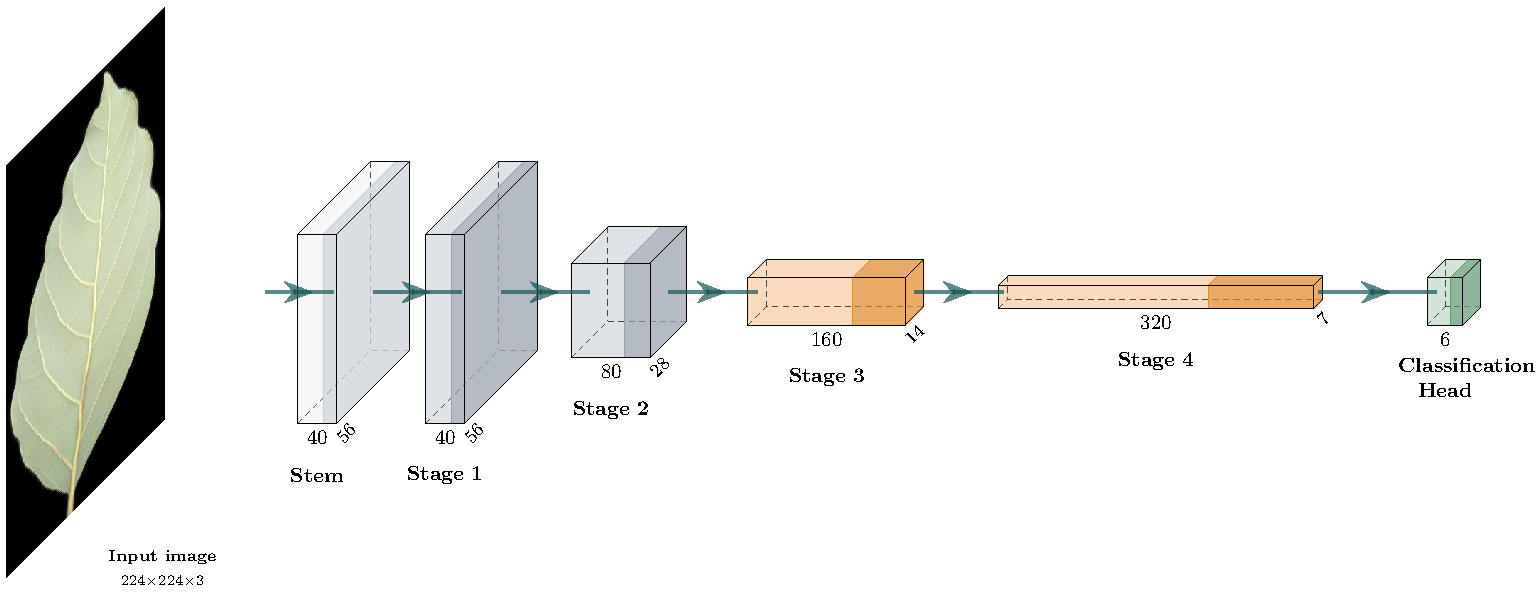
\includegraphics[width=0.75\textwidth]{img/models/proposed_architecture.pdf}
\caption{Architecture of Model BoVien. Grey indicates frozen (ImageNet-pretrained, unchanged) parameters, orange indicates parameters fine-tuned on AvocadoLeaf, and green indicates newly initialised, always-trainable parameters.}
\label{fig:proposed_architecture}
\end{figure*}
